% Provenance (never printed): see sources/outline_sources.md (Year 2: ancient massifs,
% Caledonian and Variscan belts; the Wilson cycle; supercontinents). Caledonian phases after
% McKerrow, Mac Niocaill and Dewey (2000) and Schiffer et al. (2020); the Wilson cycle after
% Chenin et al. (2018) and Schiffer et al. (2020); the Variscan belt after Faure (2024);
% supercontinents after Nance (2022); Siccar Point after the IUGS Geoheritage description.
% Model ocean and supercontinent chart from figdata/bachelor-2/wilson.py. Exercise and problem
% values in the Book 4 scratch calculator calc/ch15.py.
\chapter{Maciços antigos e o ciclo de Wilson}\label{ch:b2:wilson-cycle}

Na costa do sudeste da Escócia, em Siccar Point, camadas cinzentas de arenito estão de pé
sob uma cobertura de arenito vermelho que mergulha suavemente em direção ao mar. As camadas cinzentas foram depositadas em
um oceano no início do Siluriano, depois dobradas e clivadas quando esse oceano se fechou; foram desgastadas
até uma superfície irregular; no Devoniano Superior, cascalhos vermelhos as soterraram, e uma segunda
orogênese, mais suave, inclinou por sua vez as camadas vermelhas. Uma única falésia registra um oceano que
desapareceu, um cinturão de montanhas que se foi, e o seguinte. Este capítulo lê esses registros,
reúne-os num ciclo que as bacias oceânicas seguem, e recua até o ritmo mais longo de
todos, a reunião e a fragmentação dos \omterm{def:b2:wilson-cycle:supercontinent}{supercontinentes}.
% ledger: iugs:siccar-orogenies, iugs:siccar-point

\begin{recall}
\textbf{Dos volumes escolares}: a Pangeia e sua fragmentação, os \omterm{def:b2:wilson-cycle:supercontinent}{supercontinentes}; as discordâncias;
a taxa de denudação, a recuperação isostática e o decaimento exponencial de uma cadeia de montanhas desgastada
por seus rios. \textbf{Do volume do primeiro ano}: os riftes continentais, as margens passivas e as
dorsais meso-oceânicas, as taxas de expansão total e de meia expansão; a subducção e as margens ativas.
\textbf{Do \cref{ch:b2:crustal-melting} ao \cref{ch:b2:himalaya-andes}}: \omterm{def:b2:crustal-melting:migmatite}{migmatitos} e
granitos; \omterm{def:b2:alpine-orogen:orogen}{orógeno}, \omterm{def:b2:alpine-orogen:ophiolite}{ofiolito}, sutura, \omterm{def:b2:alpine-orogen:nappes}{nappe}, \omterm{def:b2:alpine-orogen:foreland}{flysch} e \omterm{def:b2:alpine-orogen:foreland}{molassa}, \omterm{def:b2:alpine-orogen:foreland}{bacia de antepaís}; \omterm{def:b2:himalaya-andes:types}{orógenos de colisão} e
de tipo andino; \omterm{def:b2:himalaya-andes:thickening}{espessamento crustal}, espessura de Airy e \omterm{def:b2:himalaya-andes:collapse}{colapso gravitacional}.
\end{recall}

\begin{omfigure}
\centering
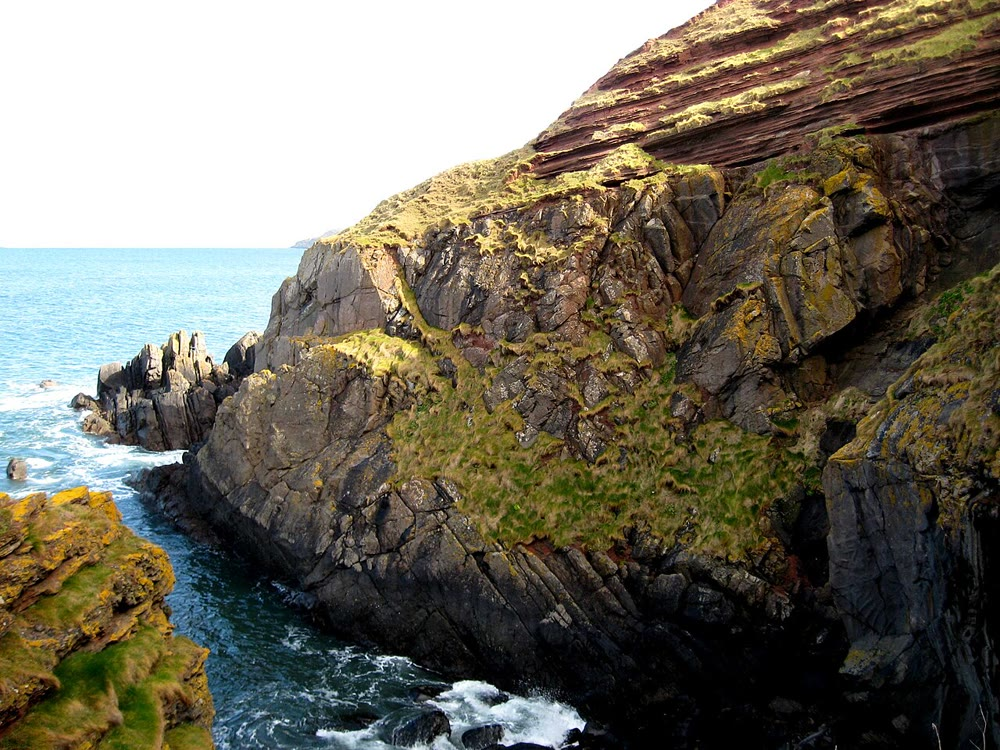
\includegraphics[width=0.64\linewidth]{images/book4/b2-15-siccar-point.jpg}
\par\smallskip{\small Siccar Point, a sudeste do promontório: camadas quase verticais de grauvaca cinzenta
siluriana, dobradas na orogenia caledoniana, sob camadas vermelhas de mergulho suave do
Devoniano Superior. Fotografia de dave souza, 2008, CC BY-SA 4.0.}
\end{omfigure}
% ledger: iugs:siccar-orogenies

\section{Cinturões desgastados até as raízes}\label{sec:b2:wilson-cycle:old}

A Europa Ocidental e o leste da América do Norte são atravessados por cinturões de montanhas muito mais antigos que os
Alpes. Seus cumes desapareceram, mas suas rochas permanecem. Três deles importam aqui.

O cinturão \emph{caledoniano} vai da Noruega, pela Escócia e pela Irlanda, até a Terra Nova e
o norte dos Apalaches, e continua pela Groenlândia Oriental e por Svalbard. Ele é o registro de um
oceano, o Iapetus, que ficava no início do Paleozoico entre a Laurentia, ancestral da América do
Norte e da Groenlândia, a noroeste, e a Báltica e a Avalônia, a sudeste e a leste.
Suas margens tinham se separado por rifteamento há cerca de 600 milhões de anos; seu fechamento, do Cambriano ao
Devoniano, produziu toda uma série de colisões, de modo que a orogenia caledoniana abrange cerca de
200 milhões de anos. O termo designa um lugar e um oceano, não uma idade.
% ledger: mckerrow00:caledonian, schiffer20:caledonides

O cinturão \emph{varisco}, chamado hercínico em textos mais antigos, atravessa a Europa do sudoeste da
Inglaterra e da Bélgica, pela França e pela Ibéria, até a Europa central; o cinturão \emph{apalachiano} do
leste da América do Norte é seu gêmeo ocidental. Juntos, eles registram o fechamento dos oceanos
entre o continente do sul, o Gondwana, e o do norte, que acabava de ser soldado pelas
colisões caledonianas. Sua última colisão, no Carbonífero Superior e no Permiano, deixou
um cinturão de dobras que corre de leste a oeste pelo sul da Europa e de nordeste a sudoeste entre
o leste da América do Norte e o noroeste da África, e com ele o \omterm{def:b2:wilson-cycle:supercontinent}{supercontinente} Pangeia.
% ledger: schiffer20:variscan, faure24:variscan

Como se reconhece um cinturão de montanhas erodido durante trezentos milhões de anos?
Não pelo seu relevo, que desapareceu. Procuram-se suas partes, cada uma das quais os capítulos
anteriores já apresentaram:
\begin{itemize}
\item \emph{suturas} marcadas por \emph{\omterm{def:b2:alpine-orogen:ophiolite}{ofiolitos}}, lascas do fundo do oceano que se fechou;
\item faixas de \emph{rochas metamórficas}, frequentemente de alto grau, as raízes da crosta espessada,
hoje na superfície porque os quilômetros acima delas foram erodidos;
\item \emph{granitos} e \emph{\omterm{def:b2:crustal-melting:migmatite}{migmatitos}}, os produtos da fusão crustal que o
espessamento e o aquecimento trazem;
\item sedimentos do oceano que se fecha e do cinturão: o \emph{\omterm{def:b2:alpine-orogen:foreland}{flysch}}, despejado em bacias profundas
durante a convergência, a \emph{\omterm{def:b2:alpine-orogen:foreland}{molassa}}, despejada em \omterm{def:b2:alpine-orogen:foreland}{bacias de antepaís} e intramontanas;
\item \emph{discordâncias angulares}, onde camadas mais jovens repousam sobre camadas dobradas e
erodidas antes delas, datando a deformação entre as duas.
\end{itemize}

\begin{definition}[Peneplanície]\label{def:b2:wilson-cycle:peneplain}
Uma \emph{peneplanície}\index{peneplanície} é uma superfície de terreno de baixo relevo, perto do nível de base da
erosão, cortada através de rochas de dureza e estrutura diferentes por uma longa erosão de um antigo
relevo.
\end{definition}

O cinturão varisco é um \omterm{def:b2:alpine-orogen:orogen}{orógeno} quente. Nos Alpes do \cref{ch:b2:alpine-orogen}, as rochas
seguiram gradientes metamórficos de cerca de \qty{8}{\celsius} por quilômetro; no cinturão varisco,
de cerca de \qty{30}{\celsius} por quilômetro. Sua crosta fundiu amplamente: no Maciço Central francês
e no Maciço Armoricano, \omterm{def:b2:crustal-melting:migmatite}{migmatitos} se formaram entre cerca de 330 e 325 milhões de anos atrás, e
granitos os intrudiram. Essa fusão é a principal diferença em relação aos Alpes Ocidentais. Quando a
colisão terminou, a crosta espessada se afinou por extensão, rochas metamórficas foram trazidas para cima
ao longo de \omterm{def:b2:alpine-orogen:decollement}{descolamentos}, e bacias intramontanas se abriram; depois, a erosão nivelou a cadeia numa
\omterm{def:b2:wilson-cycle:peneplain}{peneplanície} permiana e triássica sobre a qual foram depositados os sedimentos do ciclo seguinte.
% ledger: faure24:variscan

\begin{omfigure}
\centering\small
\begin{tabular}{>{\raggedright\arraybackslash}p{0.2\linewidth}|>{\raggedright\arraybackslash}p{0.17\linewidth}|>{\raggedright\arraybackslash}p{0.52\linewidth}}
fase & idade & o que colidiu \\ \hline
Penobscotiana & 490--485 Ma & um arco insular cavalgado sobre a margem da Avalônia \\
Grampiana, Tacônica & 480--455 Ma & arcos insulares contra a Laurentia (Escócia; norte dos Apalaches) \\
Shelveiana & início do Ordoviciano Superior & a Avalônia contra a Báltica; o mar de Tornquist se fecha \\
Escandiana & 425--400 Ma & a Báltica contra a Laurentia; as grandes \omterm{def:b2:alpine-orogen:nappes}{nappes} da Escandinávia \\
Acadiana & Devoniano Inferior & \omterm{def:b2:wilson-cycle:terrane}{terrenos} vindos do Gondwana contra o novo continente; Iapetus fechado \\
\end{tabular}
\par\smallskip{\small As principais fases da orogenia caledoniana. As primeiras fases são
colisões de arcos com arcos ou com continentes, as últimas, colisões de continentes; a maioria das
fases começou em momentos diferentes em lugares diferentes.}
\end{omfigure}
% ledger: mckerrow00:phases, schiffer20:caledonides

A tabela caledoniana acima mostra a outra marca dos cinturões antigos: eles são compostos. Antes que os
dois continentes se encontrassem, arcos e blocos menores chegaram um a um e foram soldados.

\begin{definition}[Terreno; microcontinente]\label{def:b2:wilson-cycle:terrane}
Um \emph{terreno}\index{terreno (tectônico)} é um bloco de crosta limitado por falhas cuja história geológica
difere da de seus vizinhos, trazido à sua posição atual pelo movimento das placas; ele pode
ser um arco insular, um platô oceânico, uma lasca de fundo oceânico ou um fragmento de continente. Um
\emph{microcontinente}\index{microcontinente} é um bloco de crosta continental, menor que um
continente, separado dos continentes por crosta oceânica.
\end{definition}

A Avalônia foi um bloco assim: uma faixa de crosta que deixou a margem do Gondwana, abriu o oceano
Rheic atrás de si no Ordoviciano, atravessou o Iapetus e se acoplou à Báltica e depois à
Laurentia. A Armórica e a Saxoturíngia, hoje na França e na Alemanha, a seguiram por sua vez; suas
suturas, marcadas por \omterm{def:b2:alpine-orogen:ophiolite}{ofiolitos}, dividem o cinturão varisco em zonas, de um antepaís norte
no antigo continente do norte a um antepaís sul no Gondwana.
% ledger: schiffer20:caledonides, schiffer20:variscan, faure24:variscan

\begin{omfigure}
\centering
\begin{tikzpicture}[x=0.5cm, y=0.5cm, font=\scriptsize]
\tikzset{cont/.style={fill=orange!25, draw=black!60, line width=0.4pt},
  terr/.style={fill=orange!45, draw=black!60, line width=0.4pt},
  ocn/.style={font=\scriptsize\itshape, text=blue!50!black},
  belt/.style={pattern=north east lines, pattern color=red!60!black, draw=red!60!black}}
% panel A
\begin{scope}
\fill[blue!6] (0,0) rectangle (9,8);
\draw[cont] (0.3,4.2) -- (3.0,4.0) -- (3.4,7.7) -- (0.3,7.7) -- cycle;
\node[align=center] at (1.7,6.0) {Lau-\\rentia};
\draw[cont] (6.0,5.4) -- (8.7,5.0) -- (8.7,7.7) -- (6.4,7.7) -- cycle;
\node at (7.4,6.6) {Báltica};
\draw[cont] (0.3,0.3) -- (8.7,0.3) -- (8.7,1.6) -- (0.3,1.9) -- cycle;
\node at (4.5,0.95) {Gondwana};
\draw[terr] (3.8,2.4) -- (6.6,2.2) -- (6.6,2.9) -- (3.8,3.1) -- cycle;
\node at (5.2,2.65) {Avalônia};
\node[ocn] at (4.6,5.4) {Iapetus};
\node[ocn] at (7.7,2.55) {Rheic};
\node[anchor=north west, font=\small\bfseries] at (0.1,8.9) {A: cerca de 480 Ma};
\end{scope}
% panel B
\begin{scope}[xshift=5.0cm]
\fill[blue!6] (0,0) rectangle (9,8);
\draw[cont] (0.3,3.6) -- (3.0,3.4) -- (3.4,7.7) -- (0.3,7.7) -- cycle;
\draw[cont] (3.0,3.4) -- (3.4,7.7) -- (8.7,7.7) -- (8.7,4.4) -- (5.2,4.6) -- (5.0,3.4) -- cycle;
\draw[terr] (3.0,3.4) -- (5.0,3.4) -- (5.2,4.6) -- (8.7,4.4) -- (8.7,3.6) -- (3.0,2.8) -- cycle;
\draw[red!60!black, line width=1.2pt] (3.0,3.4) -- (3.4,7.7);
\draw[red!60!black, line width=1.2pt] (5.0,3.4) -- (5.2,4.6) -- (8.7,4.4);
\node[align=center] at (1.6,5.6) {Lau-\\rentia};
\node at (6.6,5.7) {Báltica};
\node at (6.4,3.75) {Avalônia};
\node at (6.0,7.1) {\textbf{Laurússia}};
\draw[cont] (0.3,0.3) -- (8.7,0.3) -- (8.7,1.3) -- (0.3,1.5) -- cycle;
\node at (4.5,0.8) {Gondwana};
\draw[terr] (2.2,1.9) -- (3.6,1.9) -- (3.6,2.3) -- (2.2,2.3) -- cycle;
\draw[terr] (5.0,1.8) -- (6.6,1.8) -- (6.6,2.2) -- (5.0,2.2) -- cycle;
\node[ocn] at (7.7,2.3) {Rheic};
\node[anchor=north west, font=\small\bfseries] at (0.1,8.9) {B: cerca de 420 Ma};
\end{scope}
% panel C
\begin{scope}[xshift=10.0cm]
\fill[blue!6] (0,0) rectangle (9,8);
\draw[cont] (0.3,3.0) -- (8.7,3.0) -- (8.7,7.7) -- (0.3,7.7) -- cycle;
\draw[cont] (0.3,0.3) -- (8.7,0.3) -- (8.7,3.0) -- (0.3,3.0) -- cycle;
\fill[belt] (0.3,2.5) -- (8.7,2.5) -- (8.7,3.5) -- (0.3,3.5) -- cycle;
\node[fill=orange!25, inner sep=1pt] at (4.5,5.6) {Laurússia};
\node[fill=orange!25, inner sep=1pt] at (4.5,1.3) {Gondwana};
\node[fill=white, fill opacity=0.85, text opacity=1, inner sep=1pt, align=center] at (4.5,3.0)
  {cinturão Varisco--Apalachiano};
\node[ocn] at (7.6,0.7) {};
\node[anchor=north west, font=\small\bfseries] at (0.1,8.9) {C: cerca de 300 Ma, Pangeia};
\end{scope}
\end{tikzpicture}
\par\smallskip{\small Três momentos do fechamento dos oceanos Iapetus e Rheic, num
esboço esquemático sem projeção cartográfica e sem escala: posições, tamanhos e formas são apenas
topológicos. A: a Avalônia deixou o Gondwana e o oceano Rheic se abre atrás dela. B: o Iapetus se
fechou; a Laurentia, a Báltica e a Avalônia formam a Laurússia, ao longo de suturas caledonianas (linhas vermelhas);
blocos menores atravessam o oceano Rheic. C: o Gondwana encontrou a Laurússia ao longo do
cinturão Varisco--Apalachiano (hachurado).}
\end{omfigure}
% ledger: mckerrow00:caledonian, mckerrow00:phases, schiffer20:caledonides, schiffer20:variscan, faure24:variscan

\section{O ciclo de Wilson}\label{sec:b2:wilson-cycle:cycle}

Em 1966, J. Tuzo Wilson perguntou se o Atlântico tinha se fechado e depois
se aberto de novo. Fósseis do Paleozoico inferior e médio lhe diziam que um oceano largo tinha então
separado as faunas da América do Norte das da Europa Ocidental, um oceano que já não
existia do fim do Paleozoico até o meio do Mesozoico. O Atlântico moderno tinha se aberto
quase onde esse oceano mais antigo, o Iapetus, tinha se fechado.
% ledger: schiffer20:wilson, chenin18:cycle

\begin{definition}[Ciclo de Wilson]\label{def:b2:wilson-cycle:wilson}
O \emph{ciclo de Wilson}\index{ciclo de Wilson} é a sucessão de etapas pelas quais uma
bacia oceânica se abre e se fecha de novo entre margens continentais: rifteamento continental,
ruptura e expansão do fundo oceânico, um oceano que se alarga com margens passivas, o início da
subducção, o estreitamento e o fechamento do oceano, a colisão continental, e o colapso
e a erosão do cinturão, depois do qual o continente soldado pode sofrer rifteamento de novo ao longo da mesma zona.
\end{definition}

A figura abaixo acompanha as etapas. São as dos capítulos anteriores postas em ordem:
os riftes e as margens passivas do volume do primeiro ano, as margens ativas e seus arcos, as
colisões alpina e himalaiana, o \omterm{def:b2:himalaya-andes:collapse}{colapso gravitacional} do Tibete, o lento desgaste
dos cinturões antigos.

\begin{omfigure}
\centering
\begin{tikzpicture}[x=0.38cm, y=0.38cm, font=\scriptsize]
\tikzset{crust/.style={fill=orange!25, draw=black!60, line width=0.3pt},
  ocrust/.style={fill=gray!45, draw=black!60, line width=0.3pt},
  sea/.style={fill=blue!8},
  ttl/.style={anchor=west, font=\scriptsize\bfseries}}
% 1 continent
\begin{scope}
\draw[crust] (0,0) -- (16,0) -- (16,2) -- (0,2) -- cycle;
\node[ttl] at (0,3.1) {1\enspace um continente};
\end{scope}
% 2 rift
\begin{scope}[xshift=7.2cm]
\draw[crust] (0,0) -- (7,0) -- (7,2) -- (6.2,2) -- (5.4,1.0) -- (0,2) -- cycle;
\draw[crust] (9,0) -- (16,0) -- (16,2) -- (10.6,1.0) -- (9.8,2) -- (9,2) -- cycle;
\fill[red!50] (7,0) -- (9,0) -- (8.6,1.2) -- (7.4,1.2) -- cycle;
\draw[thick] (6.2,2) -- (7,0.4); \draw[thick] (9.8,2) -- (9,0.4);
\node[ttl] at (0,3.1) {2\enspace rifte};
\end{scope}
% 3 young ocean
\begin{scope}[yshift=-2.4cm]
\fill[sea] (5,2) -- (11,2) -- (11,0.6) -- (5,0.6) -- cycle;
\draw[crust] (0,0) -- (5,0) -- (6.2,0.5) -- (5,2) -- (0,2) -- cycle;
\draw[crust] (16,0) -- (11,0) -- (9.8,0.5) -- (11,2) -- (16,2) -- cycle;
\draw[ocrust] (6.2,0.5) -- (9.8,0.5) -- (9.8,0) -- (6.2,0) -- cycle;
\draw[red!70!black, thick] (8,0.5) -- (8,1.0);
\node[ttl] at (0,3.1) {3\enspace um oceano jovem};
\end{scope}
% 4 wide ocean
\begin{scope}[xshift=7.2cm, yshift=-2.4cm]
\fill[sea] (2.5,2) -- (13.5,2) -- (13.5,0.4) -- (2.5,0.4) -- cycle;
\draw[crust] (0,0) -- (2.5,0) -- (3.4,0.4) -- (2.5,2) -- (0,2) -- cycle;
\draw[crust] (16,0) -- (13.5,0) -- (12.6,0.4) -- (13.5,2) -- (16,2) -- cycle;
\draw[ocrust] (3.4,0.4) -- (12.6,0.4) -- (12.6,-0.4) -- (3.4,-0.4) -- cycle;
\draw[red!70!black, thick] (8,0.4) -- (8,0.9);
\node[anchor=north] at (3,-0.1) {passiva};
\node[anchor=north] at (13,-0.1) {passiva};
\node[ttl] at (0,3.1) {4\enspace um oceano largo};
\end{scope}
% 5 subduction begins
\begin{scope}[yshift=-4.8cm]
\fill[sea] (2.5,2) -- (13.5,2) -- (13.5,0.4) -- (2.5,0.4) -- cycle;
\draw[crust] (0,0) -- (2.5,0) -- (3.4,0.4) -- (2.5,2) -- (0,2) -- cycle;
\draw[crust] (16,-0.4) -- (13.3,-0.4) -- (12.6,0.4) -- (13.5,2) -- (16,2) -- cycle;
\draw[ocrust] (3.4,0.4) -- (12.6,0.4) -- (11.6,-1.6) -- (3.4,-0.4) -- cycle;
\fill[red!60!black] (14.2,2) -- (14.6,2.7) -- (15.0,2) -- cycle;
\draw[red!70!black, thick] (7,0.4) -- (7,0.9);
\node[anchor=north] at (13.5,-0.5) {fossa};
\node[ttl] at (0,3.1) {5\enspace a subducção começa};
\end{scope}
% 6 ocean closes
\begin{scope}[xshift=7.2cm, yshift=-4.8cm]
\fill[sea] (5.5,2) -- (10.5,2) -- (10.5,0.4) -- (5.5,0.4) -- cycle;
\draw[crust] (0,0) -- (5.5,0) -- (6.4,0.4) -- (5.5,2) -- (0,2) -- cycle;
\draw[crust] (16,-0.4) -- (11.3,-0.4) -- (10.6,0.4) -- (11.5,2.4) -- (16,2.4) -- cycle;
\draw[ocrust] (6.4,0.4) -- (10.6,0.4) -- (9.4,-1.8) -- (6.4,-0.4) -- cycle;
\fill[red!60!black] (12.4,2.4) -- (12.8,3.1) -- (13.2,2.4) -- cycle;
\node[anchor=north west] at (11.6,-0.5) {arco, fossa};
\node[ttl] at (0,3.1) {6\enspace o oceano se fecha};
\end{scope}
% 7 collision
\begin{scope}[yshift=-7.2cm]
\draw[crust] (0,0) -- (16,0) -- (16,2) -- (10,2) -- (8.6,3.6) -- (7.4,3.4) -- (6,2) -- (0,2) -- cycle;
\fill[crust] (5.6,0) -- (10.4,0) -- (9.6,-1.6) -- (6.4,-1.6) -- cycle;
\draw[black!60, line width=0.3pt] (5.6,0) -- (6.4,-1.6) -- (9.6,-1.6) -- (10.4,0);
\draw[red!60!black, line width=1pt] (8.6,3.6) -- (7.6,-1.6);
\node[anchor=west, text=red!60!black] at (9.0,3.5) {sutura};
\node[ttl] at (0,3.1) {7\enspace colisão};
\end{scope}
% 8 worn flat
\begin{scope}[xshift=7.2cm, yshift=-7.2cm]
\draw[crust] (0,0) -- (16,0) -- (16,2) -- (0,2) -- cycle;
\draw[red!60!black, line width=1pt] (8.4,2) -- (7.6,0);
\fill[pink!60!red!40] (6.0,1.0) ellipse (0.7 and 0.4);
\node[anchor=north] at (8,-0.1) {peneplanície sobre a antiga raiz};
\node[ttl] at (0,3.1) {8\enspace um cinturão aplainado; um rifte pode se seguir};
\end{scope}
\end{tikzpicture}
\par\smallskip{\small As etapas do \omterm{def:b2:wilson-cycle:wilson}{ciclo de Wilson}, em seções esquemáticas (fora de escala):
crosta continental em laranja, crosta oceânica em cinza, a dorsal em vermelho, os vulcões do arco como
triângulos; no último painel, a sutura e um granito permanecem numa crosta de espessura normal.}
\end{omfigure}
% ledger: chenin18:cycle, schiffer20:wilson

\subsection{Que largura, que duração?}

Um oceano cresce por expansão do fundo oceânico em sua dorsal e diminui por subducção em suas fossas.
Uma contabilidade simples dá sua largura.

\begin{proposition}[Largura de um oceano ao longo de um ciclo]\label{prop:b2:wilson-cycle:width}
Abra-se um oceano no instante $t_0$ e alargue-se à taxa de expansão total $V_s$ de sua dorsal, até que uma
zona de subducção comece numa margem no instante $t_1$ e consuma fundo oceânico à taxa $V_c$
em relação a essa margem, com $V_c > V_s$, a dorsal continuando a se expandir. Sua largura é
\[
  W(t) = V_s\,(t - t_0) \quad (t_0 \le t \le t_1), \qquad
  W(t) = V_s\,(t_1 - t_0) - (V_c - V_s)\,(t - t_1) \quad (t \ge t_1),
\]
máxima em $t_1$, e o oceano se fecha um tempo $V_s(t_1 - t_0)/(V_c - V_s)$ depois do início da
subducção. Com expansão simétrica, a dorsal se move em direção à fossa a $V_c - V_s/2$.
\end{proposition}

\begin{proof}
Mantenha-se fixa a margem com a fossa. Antes de $t_1$, as duas margens se afastam à taxa de expansão
total $V_s$, de modo que a largura cresce a $V_s$ a partir de zero. Depois de $t_1$, a placa entre a
fossa e a dorsal se move em direção à fossa a $V_c$; a dorsal acrescenta $V_s$ à distância
entre essa placa e a placa distante, de modo que a margem distante se move em direção à fossa a $V_c - V_s$,
a taxa à qual a largura diminui. A largura chega a zero depois de $V_s(t_1 - t_0)/(V_c -
V_s)$. Com expansão simétrica, a dorsal se move à média das velocidades das placas de
cada lado, $(V_c + (V_c - V_s))/2 = V_c - V_s/2$.
\end{proof}

A figura abaixo aplica essa contabilidade a um oceano-modelo de tipo Iapetus: expansão a partir de
\qty{570}{Ma} a \qty{30}{mm} por ano, subducção a partir de \qty{490}{Ma} consumindo \qty{60}{mm} por
ano. As taxas são hipóteses, valores redondos da ordem dos medidos hoje nos oceanos; o
Iapetus real não foi nem tão simples nem tão bem conhecido. O oceano-modelo atinge \qty{2400}{km}
e se fecha a \qty{410}{Ma}, dentro do intervalo de tempo da colisão escandiana.
% values (wilson.py): max_width_km 2400, closure_Ma 410; ledger: mckerrow00:caledonian, schiffer20:caledonides

\begin{omfigure}
\centering
% figdata/bachelor-2/wilson.py part ocean (model values: assumptions)
\begin{tikzpicture}
\begin{axis}[width=0.8\linewidth, height=5.0cm, x dir=reverse, xmin=360, xmax=600, ymin=0,
  ymax=3300, ytick={0,1000,2000,3000}, xlabel={idade (\unit{Ma})}, ylabel={largura do oceano (\unit{km})},
  tick label style={font=\scriptsize}, label style={font=\small}, xtick={600,560,...,360}]
\addplot[omThm, line width=1.2pt] table[x=t_Ma, y=width_km] {figdata/out/bachelor-2-wilson-ocean.dat};
\draw[dashed, black!50] (axis cs:490,0) -- (axis cs:490,2400);
\draw[dashed, black!50] (axis cs:570,0) -- (axis cs:570,2750);
\draw[dashed, black!50] (axis cs:410,0) -- (axis cs:410,2750);
\node[font=\scriptsize, anchor=south] at (axis cs:570,2750) {início da expansão};
\node[font=\scriptsize, anchor=south west] at (axis cs:488,2400) {início da subducção};
\node[font=\scriptsize, anchor=south] at (axis cs:410,2750) {colisão};
\node[font=\scriptsize, anchor=west] at (axis cs:540,600) {abertura a $V_s$};
\node[font=\scriptsize, anchor=south west, align=left] at (axis cs:446,1150) {fechamento\\a $V_c - V_s$};
\end{axis}
\end{tikzpicture}
\par\smallskip{\small Largura de um oceano-modelo ao longo de um \omterm{def:b2:wilson-cycle:wilson}{ciclo de Wilson}, pela
\cref{prop:b2:wilson-cycle:width}, com $V_s = \qty{30}{mm}$ por ano a partir de \qty{570}{Ma} e $V_c
= \qty{60}{mm}$ por ano a partir de \qty{490}{Ma}. O tempo corre da esquerda para a direita.}
\end{omfigure}

\subsection{Abrir-se onde se fechou}

A ideia de Wilson repousa sobre uma ideia mecânica: um cinturão antigo é uma zona fraca, e um continente
estirado tende a se romper ao longo de suas zonas fracas, em vez de através do seu interior forte e
estável.

\begin{definition}[Reativação estrutural]\label{def:b2:wilson-cycle:reactivation}
A \emph{reativação estrutural}\index{reativação estrutural} de uma estrutura preexistente
(uma falha, uma zona de cisalhamento, uma sutura, um contato litológico) é a nova concentração da
deformação ao longo dela, sob um campo de tensões posterior que pode diferir daquele que a formou.
\end{definition}

O Atlântico Norte é o caso de teste, e ele só passa em parte. No Atlântico Central, o
oceano jovem segue de perto os Apalaches. Entre a Escandinávia e a Groenlândia, a ruptura
segue em linhas gerais o cinturão caledoniano. Mais ao sul, não: a sutura do Iapetus ainda corre
pelo norte da Inglaterra e pelo centro da Irlanda, e o Atlântico se abriu a oeste dela, deixando
pedaços da antiga crosta da Laurentia na margem noroeste da Europa, em torno de Rockall e Hatton.
Mais a noroeste, o mar de Labrador e a baía de Baffin cortam diretamente crátons e cinturões
mais antigos. As estruturas antigas guiam os riftes posteriores, mas nem sempre: uma fraqueza que se resfriou por mais
de 30 a 50 milhões de anos pode ter se tornado forte, e um novo rifte pode seguir a trama mais profunda
do manto em vez da sutura crustal. O \omterm{def:b2:wilson-cycle:wilson}{ciclo de Wilson} é um guia, não uma lei.
% ledger: schiffer20:wilson, schiffer20:reactivation

Nem todo ciclo abre um oceano largo. Muitos \omterm{def:b2:alpine-orogen:orogen}{orógenos} fecham oceanos embrionários, riftes que mal tinham
começado a se expandir, com menos de cerca de \qty{500}{km} de largura: os Alpes, os Pirineus, a maior parte do
cinturão varisco da Europa ocidental. Outros fecham oceanos largos e maduros, como fizeram as Caledonides
escandinavas. A diferença aparece no fim. Um cinturão que fechou um oceano largo carregou um
arco de longa duração, que drenou do manto abaixo sua parte fusível; seu colapso foi pobre em
\omterm{def:b2:magma-emplacement:magma}{magma}, como nas Caledonides. Um cinturão que fechou uma bacia estreita repousa sobre um \omterm{def:b2:mantle-melting:fertility}{manto fértil}; seu
colapso pode ser rico em \omterm{def:b2:magma-emplacement:magma}{magma}, como no cinturão varisco, onde o Moho é hoje plano e a
crosta inferior acamadada, interpretada como basalto sobreplacado sob a crosta ou como crosta inferior cisalhada
ainda quente. Em algumas dezenas de milhões de anos, as anomalias
térmicas de um cinturão se apagam; suas estruturas permanecem.
% ledger: chenin18:cycle

\section{Supercontinentes}\label{sec:b2:wilson-cycle:supercontinents}

\begin{definition}[Supercontinente; ciclo dos supercontinentes]\label{def:b2:wilson-cycle:supercontinent}
Um \emph{supercontinente}\index{supercontinente} é uma massa de terra que reúne a maior parte da crosta
continental da Terra num único bloco. O \emph{ciclo dos supercontinentes}\index{ciclo dos supercontinentes}
é a reunião episódica dos continentes num supercontinente e sua posterior
fragmentação, repetida ao longo da história da Terra.
\end{definition}

A Pangeia, que Wegener reconstruiu e os volumes escolares descreveram, existiu de cerca de 325
a 200 milhões de anos atrás. \omterm{def:b2:wilson-cycle:supercontinent}{Supercontinentes} anteriores foram propostos: a Panótia, de cerca de 620 a
580 milhões de anos atrás, cuja existência é debatida; a Rodínia, de cerca de 950 a 800 milhões de anos atrás;
a Nuna, também chamada Columbia, de cerca de 1.6 a 1.4 bilhão de anos atrás; e, mais duvidosas, a Kenorland,
de cerca de 2.7 a 2.5 bilhões de anos atrás, e a Ur, de cerca de 3.0 bilhões de anos atrás. Eles parecem ter se
reunido e fragmentado a intervalos de cerca de meio bilhão de anos desde talvez o fim do
Arqueano. O ciclo foi relacionado às idades das orogêneses, aos picos nas idades dos
granitos e dos grãos de zircão que eles contêm, ao crescimento da crosta, às grandes províncias
ígneas, ao nível do mar e ao clima: a reunião de um \omterm{def:b2:wilson-cycle:supercontinent}{supercontinente} tende a coincidir
com um resfriamento.
% ledger: nance22:supercontinents

\begin{omfigure}
\centering
% figdata/bachelor-2/wilson.py part supercontinents; ledger: nance22:supercontinents
\begin{tikzpicture}
\begin{axis}[width=0.86\linewidth, height=4.6cm, x dir=reverse, xmin=0, xmax=3300, ymin=-0.7,
  ymax=6.5, ytick=\empty, xlabel={idade (\unit{Ma})}, tick label style={font=\scriptsize},
  label style={font=\small}, xtick={0,500,...,3000}, axis y line*=left,
  % rótulos: nós explícitos (a tabela figdata traz os nomes em inglês)
  clip=false]
\addplot[only marks, mark=*, mark size=1.6pt, omThm,
  error bars/.cd, x dir=both, x explicit, error bar style={line width=3pt, omThm!60}, error mark=none]
  table[x=mid_Ma, y=row, x error=half_Ma] {figdata/out/bachelor-2-wilson-supercontinents.dat}; \foreach \x/\y/\n in {3000/0/Ur, 2600/1/Kenorland, 1500/2/Nuna-Columbia, 875/3/Rodínia, 600/4/Panótia, 262.5/5/Pangeia} {\edef\temp{\noexpand\node[font=\noexpand\scriptsize, anchor=south, yshift=1pt] at (axis cs:\x,\y) {\n};}\temp}
\end{axis}
\end{tikzpicture}
\par\smallskip{\small Os \omterm{def:b2:wilson-cycle:supercontinent}{supercontinentes} ao longo da história da Terra, da reunião à fragmentação, conforme
datados numa revisão recente: as barras cobrem os intervalos citados (Ur é uma estimativa única), os
pontos, seus pontos médios. Panótia, Kenorland e Ur são debatidos. O tempo corre da esquerda para a direita.}
\end{omfigure}

O ciclo é realmente periódico? Os pontos médios dos intervalos no gráfico estão separados por 400,
1100, 625, 275 e 337.5 milhões de anos: em média cerca de 550, mas dispersos por um fator de
quatro. ``Cerca de meio bilhão de anos'' é uma tendência, não um relógio, e os \omterm{def:b2:wilson-cycle:supercontinent}{supercontinentes}
mais antigos se apoiam em evidências escassas.
% values (wilson.py): spacings 400 1100 625 275 337.5, mean 547.5 Myr

\section{Das montanhas às planícies}\label{sec:b2:wilson-cycle:erosion}

O que transforma um cinturão como o Himalaia nas colinas baixas da Bretanha? O volume do ensino médio
construiu um modelo: os rios desgastam uma cadeia a uma taxa proporcional à sua altitude média, $kh$,
e cada metro removido do topo é em parte devolvido pela recuperação isostática, de modo que só
a fração $f = (\rho_m - \rho_c)/\rho_m$ dele se perde como altura. A altitude média então
decai como
\[
  h(t) = h_0\,e^{-k f t} ,
\]
com a constante de tempo $\tau = 1/(kf)$. Nas grandes bacias de latitudes médias, a taxa de denudação é
proporcional ao relevo médio, e, sem soerguimento, o relevo cairia a um décimo do seu
valor em cerca de 11 milhões de anos: $k = \ln 10/11 \approx 0.21$ por milhão de anos. Com as
densidades de 2700 e \qty{3300}{kg.m^{-3}}, $f = 0.18$ e $\tau \approx \qty{26}{Myr}$: uma
cadeia de \qty{3}{km} de altura ainda tem \qty{1}{km} de altura uns 30 milhões de anos depois, e desce
abaixo de \qty{300}{m} depois de cerca de 60 milhões de anos.
% ledger: ahnert70:decay; values (wilson.py): k 0.20933 /Myr, f 0.18182, tau 26.275 Myr

A mesma recuperação explica por que os cinturões antigos expõem suas raízes. Para trazer uma crosta espessada de
$H$ a $T$ de volta ao nível do mar, toda a espessura extra $T - H$ deve ser erodida, enquanto a altitude
média era apenas $(T - H)f$: remove-se cerca de 5.5 vezes mais rocha do que a altura da
cadeia. Rochas que estavam a 20 ou \qty{30}{km} de profundidade na raiz chegam à superfície: os
\omterm{def:b2:crustal-melting:migmatite}{migmatitos}, granitos e gnaisses de alto grau dos maciços antigos, como os do Maciço
Central.
% ledger: ahnert70:decay

A cadeia varisca, cujas últimas colisões terminaram há cerca de 290 milhões de anos, tinha sido
nivelada numa \omterm{def:b2:wilson-cycle:peneplain}{peneplanície} durante o Permiano e o Triássico: dentro dos cerca de 60 milhões de anos
que o modelo dá. O colapso pode acelerar isso: a extensão de uma crosta espessada, como no
Tibete hoje, a afina diretamente, sem esperar pelos rios. E em Siccar Point, cascalhos do Devoniano Superior repousam sobre
camadas silurianas dobradas nas colisões caledonianas, sobre uma antiga superfície de terreno que ainda conserva
algum relevo entre as camadas duras e as moles.
% ledger: faure24:variscan, iugs:siccar-orogenies

\begin{inthefield}[Ler uma discordância angular]
Os geólogos que estudam uma discordância angular como a de Siccar Point começam por medir a
atitude das camadas abaixo e acima da superfície, direção e mergulho, em muitos lugares. Procuram
a polaridade das camadas inferiores, pela estratificação gradacional ou pelas marcas nas bases das camadas,
pois camadas dobradas podem estar invertidas. Examinam a própria superfície: seu relevo, a
alteração abaixo dela, os seixos das rochas mais antigas no conglomerado acima dela. Depois
datam: os fósseis mais jovens abaixo dão a idade antes da qual o dobramento não pode ter acontecido,
os fósseis mais antigos acima, a idade antes da qual ele tinha acontecido e o terreno tinha sido
desgastado. O intervalo entre os dois enquadra a orogenia. Em Siccar Point, as camadas inferiores são do início do
Siluriano e as superiores do Devoniano Superior, e o dobramento, o soerguimento e a erosão caledonianos cabem
entre elas; a suave inclinação das camadas superiores é ainda mais jovem, varisca.
\end{inthefield}
% ledger: iugs:siccar-orogenies, ics:base.Silurian, ics:base.Devonian, ics:base.Carboniferous

\section*{Exercícios}\label{sec:b2:wilson-cycle:exercises}

Dados para os exercícios: $g = \qty{9.8}{m.s^{-2}}$; densidades da crosta e do manto
\qty{2700}{kg.m^{-3}} e \qty{3300}{kg.m^{-3}}; crosta normal $H = \qty{35}{km}$; idades das
bases do Siluriano, do Devoniano e do Carbonífero 443.1, 419.6 e \qty{358.9}{Ma}, do
Triássico \qty{251.9}{Ma}.

\begin{exercise}[$\star$]\label{exo:b2:wilson-cycle:1}
As margens do Iapetus sofreram rifteamento por volta de \qty{600}{Ma}; a principal colisão caledoniana, a
escandiana, terminou por volta de \qty{400}{Ma}; a primeira colisão arco--continente com a Laurentia começou
por volta de \qty{480}{Ma}. (a) Quanto durou o ciclo inteiro do Iapetus? (b) Quanto duraram as
colisões? (c) Por que ``caledoniano'' não deve ser usado para designar uma idade?
\end{exercise}

\begin{exercise}[$\star$]\label{exo:b2:wilson-cycle:2}
Ponha estas situações na ordem do \omterm{def:b2:wilson-cycle:wilson}{ciclo de Wilson} e dê o nome da etapa de cada uma: (a) o
mar Vermelho, um oceano estreito entre margens jovens de rifte; (b) o Himalaia; (c) o rifte do
leste da África; (d) o oceano Atlântico, largo, com margens passivas dos dois lados; (e) a margem pacífica
da América do Sul; (f) as colinas baixas da Bretanha sobre um antigo embasamento de granito e gnaisse.
\end{exercise}

\begin{exercise}[$\star$]\label{exo:b2:wilson-cycle:3}
Em Siccar Point, camadas do início do Siluriano estão sob camadas do Devoniano Superior. (a) Entre que limites,
dados pelos dados acima, o dobramento, o soerguimento e a erosão devem ter ocorrido? (b) Qual é
o tempo mais longo que eles podem ter levado? (c) Liste em ordem os eventos que a falésia registra.
\end{exercise}

\begin{exercise}[$\star$]\label{exo:b2:wilson-cycle:4}
Diga se cada um é um \omterm{def:b2:wilson-cycle:terrane}{terreno}, um \omterm{def:b2:wilson-cycle:terrane}{microcontinente}, os dois ou nenhum, e por quê: (a) a Avalônia;
(b) a Laurentia; (c) um arco insular acrescido a um continente; (d) a sutura do Iapetus.
\end{exercise}

\begin{exercise}[$\star\star$]\label{exo:b2:wilson-cycle:5}
Tome os pontos médios dos intervalos dos \omterm{def:b2:wilson-cycle:supercontinent}{supercontinentes} Ur (3000), Kenorland (2600),
Nuna (1500), Rodínia (875), Panótia (600) e Pangeia (262.5), em milhões de anos atrás.
(a) Calcule os cinco espaçamentos e sua média. (b) Qual é a razão entre o maior espaçamento e
o menor? (c) Descarte Kenorland e Ur, que são duvidosos: qual é o espaçamento médio dos
outros quatro? ``Meio bilhão de anos'' é um período?
\end{exercise}

\begin{exercise}[$\star\star$]\label{exo:b2:wilson-cycle:6}
Um oceano de \qty{3000}{km} de largura começa a ser subductado numa margem a \qty{70}{mm} por ano,
enquanto sua dorsal se expande a \qty{25}{mm} por ano. (a) Quanto tempo ele leva para se fechar?
(b) Quanto tempo, se a expansão parar imediatamente? (c) O movimento de que placa fixa a taxa de fechamento depois
que a dorsal foi subductada?
\end{exercise}

\begin{exercise}[$\star\star$]\label{exo:b2:wilson-cycle:7}
Suponha que a fusão crustal comece a cerca de \qty{700}{\celsius} e que a superfície esteja a
\qty{0}{\celsius}. (a) A que profundidade essa temperatura é atingida ao longo de um gradiente de
\qty{8}{\celsius} por quilômetro? E de \qty{30}{\celsius} por quilômetro? (b) Que cinturão, os
Alpes ou o cinturão varisco, deveria então expor \omterm{def:b2:crustal-melting:migmatite}{migmatitos} e granitos de origem crustal?
(c) Por que um gradiente fixo superestima a profundidade no primeiro caso?
\end{exercise}

\begin{exercise}[$\star\star$]\label{exo:b2:wilson-cycle:8}
As colisões variscas terminaram por volta de \qty{290}{Ma}; uma \omterm{def:b2:wilson-cycle:peneplain}{peneplanície} tinha se formado no Permiano e no
Triássico. Use o modelo de decaimento do capítulo, $\tau = \qty{26.3}{Myr}$. (a) Quanto tempo uma
cadeia leva para cair de uma altitude média de \qty{3}{km} para \qty{0.3}{km}? (b) A que idade isso
corresponderia? (c) Que constante de tempo a levaria até lá na base do Triássico? (d) Que
processo pode encurtar esse tempo?
\end{exercise}

\begin{exercise}[$\star\star$]\label{exo:b2:wilson-cycle:9}
(a) Explique por que a sutura do Iapetus no norte da Inglaterra e no centro da Irlanda, e a crosta
laurenciana perto de Rockall, mostram que o Atlântico não se reabriu exatamente ao longo da antiga sutura.
(b) O que um geólogo esperaria encontrar no antigo embasamento de cada lado da sutura
na Irlanda? (c) Os Apalaches foram deformados até o Permiano Inferior; o rifteamento começou
cerca de 80 milhões de anos depois da orogenia. Compare com os 30 a 50 milhões de anos depois dos quais
uma zona resfriada pode estar forte demais para ser reativada.
\end{exercise}

\begin{exercise}[$\star\star\star$]\label{exo:b2:wilson-cycle:10}
Um oceano de \qty{3000}{km} de largura tem sua dorsal no meio, a \qty{1500}{km} de uma fossa que
consome a placa do seu lado a \qty{70}{mm} por ano; a dorsal se expande a \qty{40}{mm} por
ano, simetricamente. (a) A que velocidade a dorsal se aproxima da fossa? (b) Quando ela a
atinge? (c) Que largura tem o oceano nesse momento? (d) O que acontece com o arco vulcânico quando uma dorsal é
subductada?
\end{exercise}

\begin{exercise}[$\star\star\star$]\label{exo:b2:wilson-cycle:11}
Uma colisão espessa uma crosta de \qty{35}{km} para \qty{60}{km}, compensada à maneira de Airy.
(a) Qual é a altitude média, pela \cref{prop:b2:himalaya-andes:airy}? (b) Quanta rocha a erosão
deve remover para trazer a superfície de volta ao nível do mar com uma crosta de espessura normal?
(c) Qual era a pressão litostática sobre as rochas que terminam na superfície? (d) Em que
\omterm{def:b2:metamorphic-facies:facies}{fácies metamórfica} elas podem ter se recristalizado?
\end{exercise}

\begin{exercise}[$\star\star\star$]\label{exo:b2:wilson-cycle:12}
Depois que dois continentes se encontram, a convergência continua a \qty{30}{mm} por ano durante \qty{10}{Myr}. O
encurtamento é absorvido através de um cinturão que termina com \qty{300}{km} de largura, numa crosta que tinha
\qty{35}{km} de espessura. (a) Usando a \cref{prop:b2:himalaya-andes:shortening}, encontre a espessura
crustal. (b) Encontre a altitude e a raiz de Airy. (c) Usando a \cref{prop:b2:himalaya-andes:gpe},
calcule a energia potencial excedente e compare-a com a do Tibete, \qty{6.1e12}{N.m^{-1}}.
(d) O que deveria acontecer em seguida?
\end{exercise}

\begin{problem}[{Problema de fim de semana --- o Iapetus do nascimento à morte}]\label{pb:b2:wilson-cycle:1}
Um oceano-modelo de tipo Iapetus se abre entre dois continentes, L a noroeste e B a
sudeste. O rifteamento começa a \qty{610}{Ma}; a expansão do fundo oceânico, a \qty{580}{Ma}.
Salvo indicação contrária, $g = \qty{9.8}{m.s^{-2}}$, $\rho_c = \qty{2700}{kg.m^{-3}}$, $\rho_m =
\qty{3300}{kg.m^{-3}}$ e a crosta normal tem $H = \qty{35}{km}$ de espessura. A expansão é
simétrica e sua taxa, constante.

\medskip
\noindent\textbf{Parte I --- Abertura.}
\begin{enumerate}
\item A \qty{500}{Ma}, o fundo oceânico formado a \qty{540}{Ma} está a \qty{720}{km} do eixo
da dorsal. Calcule a taxa de meia expansão em milímetros por ano.
\item Deduza a taxa de expansão total. A que classe de dorsal ela pertence, entre as dorsais lentas,
rápidas e ultralentas?
\item Que largura tinha o oceano a \qty{540}{Ma}?
\item Que largura tinha ele a \qty{500}{Ma}?
\item O que o modelo supôs para obter essas larguras?
\item Que idade tem o fundo oceânico mais antigo a \qty{500}{Ma}, e onde ele fica? Por que é um
lugar provável para o início da subducção?
\end{enumerate}

\noindent\textbf{Parte II --- Fechamento.} A \qty{500}{Ma}, uma zona de subducção começa ao longo da
margem de L e consome fundo oceânico a \qty{64}{mm} por ano em relação a L; a dorsal continua
a se expandir.
\begin{enumerate}[resume]
\item A que taxa o oceano se estreita?
\item Se a dorsal se expandisse até o fim, quando o oceano se fecharia?
\item A dorsal começa no meio do oceano. Quando ela atinge a fossa?
\item Que largura tem o oceano nesse momento?
\item Depois que a dorsal desceu, a expansão para e B se aproxima de L a \qty{40}{mm} por
ano. Quando o oceano se fecha?
\item Compare com as idades da fase escandiana, de 425 a \qty{400}{Ma}.
\end{enumerate}

\noindent\textbf{Parte III --- Colisão.} Depois da colisão, a convergência continua a
\qty{40}{mm} por ano durante \qty{8}{Myr}; o encurtamento é absorvido através de um cinturão que termina com
\qty{400}{km} de largura.
\begin{enumerate}[resume]
\item Quanto encurtamento é isso?
\item Usando a \cref{prop:b2:himalaya-andes:shortening}, encontre a espessura da crosta.
\item Usando a \cref{prop:b2:himalaya-andes:airy}, encontre sua altitude média de Airy e sua raiz.
\item Calcule sua energia potencial excedente e compare-a com a do Tibete,
\qty{6.1e12}{N.m^{-1}}.
\item O que você espera que o cinturão faça em seguida?
\end{enumerate}

\noindent\textbf{Parte IV --- Desgaste.} Por volta de \qty{410}{Ma}, o colapso baixou a altitude
média para \qty{3.0}{km}. A erosão segue então o modelo do capítulo, com $k = \ln
10/11$ por milhão de anos e recuperação isostática.
\begin{enumerate}[resume]
\item Calcule $f$ e a constante de tempo $\tau$.
\item Qual é a altitude média a \qty{380}{Ma}?
\item Quando a altitude média cai abaixo de \qty{500}{m}?
\item Quanta crosta extra é removida enquanto ela cai de \qty{3.0}{km} para \qty{0.5}{km}?
\item Que pressão litostática as rochas então expostas suportavam na raiz?
\item Sedimentos do Devoniano Superior repousam sobre o cinturão erodido em Siccar Point. O cronograma do modelo é
coerente com isso, dada a base do Carbonífero a \qty{358.9}{Ma}?
\item Para resumir: qual foi a maior largura que o oceano-modelo atingiu, em quilômetros?
\end{enumerate}
\end{problem}
